\section{Curvature diagnostic}\label{app:curvature}

% Evidence-label macros; the main preamble normally defines them.
\providecommand{\official}{\textsc{Official}}
\providecommand{\historical}{\textsc{Historical}}
\providecommand{\measurement}{\textsc{Measurement}}
\providecommand{\reproduction}{\textsc{Reproduction}}

The curvature proposals differentiate a legacy surrogate $J_B$
(Appendix~\ref{app:alg-laneb}) twice with automatic differentiation (AD). This
appendix reports a \measurement{} of that operator at one saved endpoint, IBM01 after
the first curvature stage (E74), together with the \historical{} stage records it comes
from. The finding is as follows. The AD Hessian-vector product is the Hessian of the
branch of $J_B$ that is active at the endpoint, that is, of the smooth piece of the
piecewise function that contains it. Symmetric finite differences straddle density
and RUDY branch boundaries that lie within $10^{-7}\,\mu$m of the endpoint, so they
measure jumps in the gradient rather than curvature. On the smooth wirelength term the
two agree to about $4\times10^{-9}$. $J_B$ therefore has no classical Hessian at this
endpoint, and its negative eigenvalue, $-0.442458$, describes the active branch:
a legitimate source of candidate directions, not a curvature of the score.

Negative active-branch eigenvalues are expected from the form of $J_B$. Within one
branch, the overlap of a rectangle with a grid cell is a product
$o_x(x_i)\,o_y(y_i)$ of two piecewise-linear factors, whose $2\times2$ Hessian block
in $(x_i,y_i)$ has the form $\bigl(\begin{smallmatrix}0&c\\c&0\end{smallmatrix}\bigr)$
with eigenvalues $\pm|c|$. The density and RUDY terms are sums of such products, and
only the convex wirelength term can offset them. The 13 Ritz values of the probe's
Krylov space run from $-0.442$ to $+0.354$, nearly symmetric about zero.

\subsection{IBM01 endpoint probe}\label{app:curvature-probe}

% Generated by scripts/render_publication_curvature.py from saved JSON; do not edit.
The probe evaluates the frozen legacy curvature surrogate $J_B$ at the saved IBM01 endpoint of the first curvature stage, in float32 and without any optimization or legalization. At that point $J_B=0.86905$ and $\lVert\nabla J_B\rVert_2=8.09\times10^{-2}\,\mu\mathrm{m}^{-1}$. A Lanczos run capped at 14 Hessian-vector products (HVPs) of the automatic-differentiation (AD) operator returned Rayleigh quotient $-0.442458$ with residual norm $3.49\times10^{-7}$. The historical cascade recorded the smallest eigenvalue $-0.442458$ at the same endpoint; the two values differ by $1.49\times10^{-7}$.

Let $x$ be the saved coordinate vector, $g_{\mathrm{AD}}(x)$ its AD gradient, and $H_{\mathrm{AD}}v$ the AD HVP for a unit vector $v$ over the movable coordinates. The central differences are
\[d_{\mathrm{FD}}(\epsilon)=\frac{J_B(x+\epsilon v)-J_B(x-\epsilon v)}{2\epsilon},\qquad k_{\mathrm{FD}}(\epsilon)=v^\top\frac{g_{\mathrm{AD}}(x+\epsilon v)-g_{\mathrm{AD}}(x-\epsilon v)}{2\epsilon}.\]
Positions and $\epsilon$ are in micrometers, so slopes are in $\mu\mathrm{m}^{-1}$ and curvatures in $\mu\mathrm{m}^{-2}$; the surrogate itself is dimensionless.

\begin{table}[htbp]
\centering\footnotesize
\caption{Float32 central differences along two seeded random unit directions at the saved IBM01 endpoint, all movable coordinates included. The AD columns are the slope and curvature of the branch active at $x$; the FD columns sample both sides of nearby branch boundaries. Slopes are in $\mu\mathrm{m}^{-1}$ and curvatures in $\mu\mathrm{m}^{-2}$. The directions are independent of the Lanczos vector.}
\label{tab:ibm01-curvature-diagnostic}
\begin{tabular}{@{}rrrrrr@{}}
\toprule
Dir. & $\epsilon$ ($\mu$m) & $g_{\mathrm{AD}}^\top v$ & $d_{\mathrm{FD}}$ & $v^\top H_{\mathrm{AD}}v$ & $k_{\mathrm{FD}}$ \\
\midrule
1 & $1.00\times10^{-3}$ & $-1.33\times10^{-4}$ & $-5.36\times10^{-4}$ & $3.44\times10^{-3}$ & $-2.88\times10^{-1}$ \\
1 & $3.00\times10^{-3}$ & $-1.33\times10^{-4}$ & $-5.66\times10^{-4}$ & $3.44\times10^{-3}$ & $-1.01\times10^{-1}$ \\
1 & $1.00\times10^{-2}$ & $-1.33\times10^{-4}$ & $-5.33\times10^{-4}$ & $3.44\times10^{-3}$ & $-1.28\times10^{-2}$ \\
1 & $3.00\times10^{-2}$ & $-1.33\times10^{-4}$ & $-5.00\times10^{-4}$ & $3.44\times10^{-3}$ & $9.50\times10^{-3}$ \\
1 & $1.00\times10^{-1}$ & $-1.33\times10^{-4}$ & $-5.35\times10^{-4}$ & $3.44\times10^{-3}$ & $1.82\times10^{-2}$ \\
2 & $1.00\times10^{-3}$ & $-7.68\times10^{-4}$ & $-3.28\times10^{-4}$ & $4.93\times10^{-4}$ & $-3.12\times10^{-2}$ \\
2 & $3.00\times10^{-3}$ & $-7.68\times10^{-4}$ & $-2.09\times10^{-4}$ & $4.93\times10^{-4}$ & $2.07\times10^{-3}$ \\
2 & $1.00\times10^{-2}$ & $-7.68\times10^{-4}$ & $-1.88\times10^{-4}$ & $4.93\times10^{-4}$ & $1.49\times10^{-2}$ \\
2 & $3.00\times10^{-2}$ & $-7.68\times10^{-4}$ & $-2.17\times10^{-4}$ & $4.93\times10^{-4}$ & $1.71\times10^{-2}$ \\
2 & $1.00\times10^{-1}$ & $-7.68\times10^{-4}$ & $-3.15\times10^{-4}$ & $4.93\times10^{-4}$ & $2.09\times10^{-2}$ \\
\bottomrule
\end{tabular}
\end{table}

For the full vectors, with $h_{\mathrm{FD}}=[g_{\mathrm{AD}}(x+\epsilon v)-g_{\mathrm{AD}}(x-\epsilon v)]/(2\epsilon)$, the relative difference $\lVert h_{\mathrm{FD}}-H_{\mathrm{AD}}v\rVert_2/\lVert H_{\mathrm{AD}}v\rVert_2$ ranges from 7.96 to 776 over the ten rows, and the cosine between the two vectors from $-1.36\times10^{-1}$ to $6.74\times10^{-2}$. At the endpoint, 21 coordinates sit at or beyond a canvas clamp. For direction~1 at $\epsilon=10^{-3}\,\mu$m the forward and backward cost slopes are $-8.34\times10^{-4}$ and $-2.38\times10^{-4}\,\mu\mathrm{m}^{-1}$, so the two sides already lie on different branches.

% Follow-up source: writeup/data/publication/curvature_followup_ibm01.json.
\paragraph{Precision and branch follow-up.} A separate saved probe restricts both directions to the 2{,}233 coordinates whose canvas clearance exceeds $0.1\,\mu$m in both precisions, so no perturbation can cross a canvas clamp. All forward floating operations run in float64; stored float32 constants are promoted without regeneration. With $P$ selecting these coordinates, the comparison uses $PH_{\mathrm{AD}}Pv$ and differences of $Pg_{\mathrm{AD}}$. The frozen composite is also split into its three weighted primitives, which reproduce the composite value, slope and curvature to $10^{-14}$. Table~\ref{tab:ibm01-curvature-followup} reports the gradient jump $\lVert P[g(x+\epsilon v)-g(x-\epsilon v)]\rVert_2$ in $\mu\mathrm{m}^{-1}$.

\begin{table}[htbp]
\centering\footnotesize
\caption{Guarded float64 follow-up at the saved IBM01 endpoint: gradient jump across $\pm\epsilon$ (in $\mu\mathrm{m}^{-1}$) and the relative difference between the finite-difference and AD Hessian-vector products at $\epsilon=10^{-5}\,\mu$m. A smooth term has a jump proportional to $\epsilon$; a jump that does not shrink with $\epsilon$ marks a branch boundary.}
\label{tab:ibm01-curvature-followup}
\begin{tabular}{@{}llrrrr@{}}
\toprule
Dir. & Term & $\epsilon=10^{-7}$ & $\epsilon=10^{-5}$ & $\epsilon=10^{-3}$ & Rel.\ HVP diff. \\
\midrule
1 & Wirelength & $1.51\times10^{-10}$ & $1.51\times10^{-8}$ & $1.51\times10^{-6}$ & $3.91\times10^{-9}$ \\
1 & $\tfrac12\times$density & $6.01\times10^{-3}$ & $2.20\times10^{-2}$ & $3.85\times10^{-2}$ & $4.52\times10^{5}$ \\
1 & $\tfrac12\times$RUDY & $2.50\times10^{-3}$ & $2.61\times10^{-3}$ & $2.61\times10^{-3}$ & $5.17\times10^{3}$ \\
1 & Composite $J_B$ & $6.51\times10^{-3}$ & $2.22\times10^{-2}$ & $3.86\times10^{-2}$ & $4.33\times10^{4}$ \\
\addlinespace
2 & Wirelength & $1.54\times10^{-10}$ & $1.54\times10^{-8}$ & $1.54\times10^{-6}$ & $3.45\times10^{-9}$ \\
2 & $\tfrac12\times$density & $6.01\times10^{-3}$ & $2.15\times10^{-2}$ & $3.84\times10^{-2}$ & $4.11\times10^{5}$ \\
2 & $\tfrac12\times$RUDY & $2.50\times10^{-3}$ & $2.61\times10^{-3}$ & $2.17\times10^{-2}$ & $3.98\times10^{3}$ \\
2 & Composite $J_B$ & $6.51\times10^{-3}$ & $2.16\times10^{-2}$ & $4.42\times10^{-2}$ & $3.28\times10^{4}$ \\
\bottomrule
\end{tabular}
\end{table}

Inside the guarded region the wirelength gradient changes in proportion to $\epsilon$, and its finite-difference HVP agrees with the AD product to $3.91\times10^{-9}$ and $3.45\times10^{-9}$ at $\epsilon=10^{-5}\,\mu$m. The density and RUDY gradients jump by amounts that persist down to $\epsilon=10^{-7}\,\mu$m, where the $\pm\epsilon$ samples already differ in 311 recorded min/max/clamp comparisons of the composite in each direction. At $\epsilon=10^{-3}\,\mu$m the composite jump norms are $3.86\times10^{-2}$ and $4.42\times10^{-2}$, and the relative HVP differences are 752.48 and 670.50.


\subsection{Stage records and endpoint validity}\label{app:curvature-stages}

Table~\ref{tab:curvature-stages} gives the per-design records of the two curvature
stages of the v1 lineage. They come from staged research runs without the one-hour
limit: the first stage took up to 4,007\,s (66.8 minutes) on one design and the
cascade up to 3,454\,s (57.6 minutes), in both cases on top of the time needed to
reach the plateau. In the first stage, 190 of 204 perturb-and-polish attempts ended
below the plateau with zero overlap, with nearly equal success for the first and
second eigenvectors (94 and 96 of 102) and for the step lengths 0.3, 1 and $3\,\mu$m
(64, 65 and 61 of 68). The attempts are 12 on each of 17 designs, so they are not
independent; the main text discusses what the pattern implies.

\begin{table}[htbp]
\centering
\footnotesize
\caption{Historical records from uncapped research runs (no one-hour limit). Proxy cost after each curvature stage (lower is better); the plateau is the better of the two v1 branches. Validity is a strict canvas check of the saved endpoints (Measurement); every failure exceeds a canvas edge by at most $7.63\times10^{-6}\,\mu$m and no endpoint has a hard-macro overlap.}
\label{tab:curvature-stages}
\begin{tabular}{lrrrcr}
\toprule
Design & Plateau & \shortstack{After first\\curvature stage} & \shortstack{After\\cascade} & \shortstack{Strict validity\\(first / cascade)} & \shortstack{Cascade stage\\time (s)} \\
\midrule
IBM01 & 0.88960 & 0.85527 & 0.84528 & $\checkmark$ / $\checkmark$ & 2{,}913 \\
IBM02 & 1.11890 & 1.03907 & 1.02104 & $\checkmark$ / $\checkmark$ & 3{,}285 \\
IBM03 & 0.95849 & 0.95214 & 0.94634 & $\checkmark$ / $\times$ & 3{,}431 \\
IBM04 & 1.00156 & 0.99225 & 0.99066 & $\checkmark$ / $\checkmark$ & 375 \\
IBM06 & 1.15276 & 1.13127 & 1.11792 & $\checkmark$ / $\checkmark$ & 3{,}298 \\
IBM07 & 1.09397 & 1.07574 & 1.06449 & $\times$ / $\times$ & 3{,}381 \\
IBM08 & 1.11106 & 1.10606 & 1.10069 & $\checkmark$ / $\checkmark$ & 3{,}319 \\
IBM09 & 0.82828 & 0.82735 & 0.82269 & $\times$ / $\times$ & 3{,}360 \\
IBM10 & 1.00051 & 0.99155 & 0.98940 & $\checkmark$ / $\checkmark$ & 2{,}880 \\
IBM11 & 0.87824 & 0.87293 & 0.86808 & $\checkmark$ / $\checkmark$ & 3{,}454 \\
IBM12 & 1.20534 & 1.20058 & 1.19766 & $\checkmark$ / $\checkmark$ & 3{,}432 \\
IBM13 & 0.95540 & 0.94883 & 0.93458 & $\times$ / $\times$ & 3{,}413 \\
IBM14 & 1.21609 & 1.20940 & 1.20630 & $\checkmark$ / $\checkmark$ & 3{,}284 \\
IBM15 & 1.16172 & 1.15612 & 1.15510 & $\times$ / $\times$ & 2{,}733 \\
IBM16 & 1.12347 & 1.11320 & 1.10847 & $\times$ / $\times$ & 3{,}287 \\
IBM17 & 1.33708 & 1.33323 & 1.33162 & $\checkmark$ / $\times$ & 3{,}423 \\
IBM18 & 1.34934 & 1.34419 & 1.33994 & $\checkmark$ / $\checkmark$ & 3{,}340 \\
\midrule
Mean & 1.08128 & 1.06760 & 1.06119 & 12 / 10 of 17 & 3{,}095 \\
\bottomrule
\end{tabular}
\end{table}


All 34 saved endpoints (first stage and cascade on 17 designs) were rescored with the
canonical evaluator for this report. The fresh scores reproduce the recorded ones to
within $9.87\times10^{-8}$, so every recorded decrease persists, and none of the 34
placements has a hard-macro overlap. A strict geometry check, which also requires
every rectangle to lie inside the canvas, accepts 22 of the 34: 12 of the 17
first-stage endpoints and 10 of the 17 cascade endpoints. In each of the 12 failures
an object extends past the upper canvas edge by exactly one float32 rounding step at
the canvas size: $3.81\times10^{-6}\,\mu$m on canvases of 32 to $64\,\mu$m (IBM03, IBM07,
IBM09, IBM13) and $7.63\times10^{-6}\,\mu$m on canvases of 64 to $128\,\mu$m (IBM15,
IBM16, IBM17). The excess is consistent with clipping in float64 followed by
conversion to float32; the corrected runtime instead steps a rounded-up coordinate
one representable value inward (Appendix~\ref{app:verification}). The coordinates
were left as saved, so the stage means include the 12 strictly invalid placements. On
the 10 designs whose two endpoints both pass, the mean falls from 1.074258 to
1.067697 ($-0.61\%$), lower on all 10.

\begin{figure}[htbp]
\centering
\sbox{\sidefigbox}{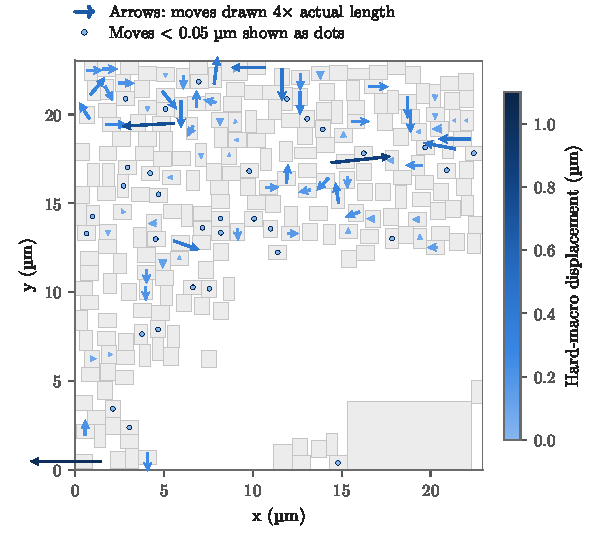
\includegraphics{figures/ibm01_displacement.pdf}}%
\begin{minipage}[c]{\wd\sidefigbox}\usebox{\sidefigbox}\end{minipage}\hfill
\begin{minipage}[c]{\dimexpr\linewidth-\wd\sidefigbox-1.2em\relax}
\captionsetup{justification=raggedright,singlelinecheck=false}
\caption{Hard-macro displacement on IBM01 between the saved endpoints of the first
curvature stage (proxy 0.85527) and the cascade (proxy 0.84528), \historical. Arrows
start at the first-stage position and are drawn four times longer than the actual
displacement, moves under $0.05\,\mu$m are drawn as dots, and color gives the
length. The difference includes the CD polish after
every accepted step, so it is not a trajectory.}
\label{fig:ibm01-displacement}
\end{minipage}
\end{figure}

Figure~\ref{fig:ibm01-displacement} shows what the cascade changed on IBM01, a design
whose two endpoints are both strictly valid. It moved 104 of the 246 hard macros, by at
most $1.01\,\mu$m on a canvas $23\,\mu$m wide; the median displacement among the moved
macros is $0.085\,\mu$m. It also moved 407 of the 894 soft clusters, by up to
$8.4\,\mu$m (not drawn). The score fell by 0.00999 through many small, scattered
adjustments rather than a rearrangement of blocks.
